%%%%%%%%%%%%%%%%%%%%%%%%%%%%%%%%%%%%%%%%%
% Short Sectioned Assignment
% LaTeX Template
% Version 1.0 (5/5/12)
%
% This template has been downloaded from:
% http://www.LaTeXTemplates.com
%
% Original author:
% Frits Wenneker (http://www.howtotex.com)
%
% License:
% CC BY-NC-SA 3.0 (http://creativecommons.org/licenses/by-nc-sa/3.0/)
%
%%%%%%%%%%%%%%%%%%%%%%%%%%%%%%%%%%%%%%%%

%----------------------------------------------------------------------------------------
%	PACKAGES AND OTHER DOCUMENT CONFIGURATIONS
%----------------------------------------------------------------------------------------

\documentclass[paper=a4, fontsize=12pt, xcolor=dvipsnames, parskip=full]{scrartcl} % A4 paper and 11pt font size

% Biblatex
\usepackage[
style=nature,              % Zitierstil
isbn=false,                % ISBN nicht anzeigen, gleiches geht mit nahezu allen anderen Feldern
pagetracker=true,          % ebd. bei wiederholten Angaben (false=ausgeschaltet, page=Seite, spread=Doppelseite, true=automatisch)
maxbibnames=50,            % maximale Namen, die im Literaturverzeichnis angezeigt werden (ich wollte alle)
maxcitenames=3,            % maximale Namen, die im Text angezeigt werden, ab 4 wird u.a. nach den ersten Autor angezeigt
autocite=inline,           % regelt Aussehen für \autocite (inline=\parancite)
block=space,               % kleiner horizontaler Platz zwischen den Feldern
backref=false,              % Seiten anzeigen, auf denen die Referenz vorkommt
backrefstyle=three+,       % fasst Seiten zusammen, z.B. S. 2f, 6ff, 7-10
date=short,                % Datumsformat
hyperref=true,
backend=biber
]{biblatex}
\setlength{\bibitemsep}{1em}     % Abstand zwischen den Literaturangaben
\setlength{\bibhang}{2em}        % Einzug nach jeweils erster Zeile
\bibliography{ba_thesis}  % Bibtex-Datei wird schon in der Preambel eingebunden
\usepackage{cmbright}
\usepackage[T1]{fontenc} % Use 8-bit encoding that has 256 glyphs

\usepackage{amsmath, amsfonts, amsthm} % Math packages
\usepackage{pgfplots}
\usepackage{wrapfig}
\usepackage{color, colortbl}  

% Bibliographie auf deutsch
\definecolor{gray1}{gray}{0.2}
\usepackage[font={color=gray1}, figurename=Fig., labelfont={color=blue}]{caption}

\usepackage{titlesec}

\usepackage[utf8]{inputenc} 
\usepackage{forloop}

\usepackage{latexsym}
\usepackage{textcomp}
\usepackage{bm}% bold math
\usepackage{graphicx}
\usepackage{eso-pic}
\usepackage{caption}
\usepackage{subcaption}
\usepackage{verbatim}
\usepackage{epsfig}
\usepackage{framed,color}
\usepackage{placeins}   % FloatBarrier
\usepackage{float}
\usepackage{sidecap}
%\usepackage{float}      % adding boxes around figures
%\floatstyle{boxed}
%\restylefloat{figure}
\usepackage[usenames,dvipsnames]{pstricks}
\usepackage{epsfig}
\usepackage{tikz}
\usepackage{sectsty} % Allows customizing section commands
\usepackage{hyperref}
\usepackage{array}
\usepackage{diagbox, pict2e}


%\usepackage[pass,showframe]{geometry} % just to show the margins
%\usepackage{booktabs}
%\usepackage{minted} % needs '-shell-escape' to compile

\listfiles
\hypersetup{
     colorlinks   = true,
     citecolor    = gray,
     linkcolor    = blue
}

\allsectionsfont{ \color{gray1} \normalfont\scshape} % Make all sections centered, the default font and small caps

\usepackage{fancyhdr} % Custom headers and footers
\pagestyle{fancy} % Makes all pages in the document conform to the custom headers and footers

\renewcommand{\headrulewidth}{0.0pt} % Remove header underlines
\renewcommand{\footrulewidth}{0pt} % Remove footer underlines

\numberwithin{equation}{section} % Number equations within sections (i.e. 1.1, 1.2, 2.1, 2.2 instead of 1, 2, 3, 4)
\numberwithin{figure}{section} % Number figures within sections (i.e. 1.1, 1.2, 2.1, 2.2 instead of 1, 2, 3, 4)
\numberwithin{table}{section} % Number tables within sections (i.e. 1.1, 1.2, 2.1, 2.2 instead of 1, 2, 3, 4)

\setlength\parindent{0pt} % Removes all indentation from paragraphs - comment this line for an assignment with lots of text
\setcapindent{1cm} 

%----------------------------------------------------------------------------------------
%	TITLE SECTION
%----------------------------------------------------------------------------------------
\title{
\normalfont \normalsize 
\textsc{Albert-Ludwigs-University Freiburg} \\ [25pt] % Your university, school and/or department name(s)
\horrule{0.5pt} \\[0.4cm] % Thin top horizontal rule
\huge \textsc{A network model of the neocortex} \\ % The assignment title
\horrule{2pt} \\[0.5cm] % Thick bottom horizontal rule
}

\author{Friedrich Schüßler} % Your name

\date{\normalsize\today} % Today's date or a custom date
\DeclareGraphicsExtensions{.png,.pdf,.jpg,.eps}

%--------------------------------------------------------------------------------------------
% New Commands
%--------------------------------------------------------------------------------------------
\newcommand{\horrule}[1]{\color{gray1}\rule{\linewidth}{#1}} % Create horizontal rule command with 1 argument of height

% Right aligned table cells with fixed length; e.g. x{2.5cm}
\newcolumntype{x}[1]{%
>{\raggedleft\hspace{0pt}}p{#1}}%
\newcommand{\tn}{\tabularnewline}
\newcommand{\tnn}{\tabularnewline[0.3cm]} % newline for costume table cells 

\definecolor{TableColor}{rgb}{0.88,0.8,1}

\renewcommand{\figdir}{../../analysis/figures/} % figure directory



%----------------------------------------------------------------------------------------
\begin{document}

\color{gray1}
\maketitle
%\begin{center}
% \includegraphics[width=0.6\linewidth]{figures/unifreiburg}
%\end{center}
\thispagestyle{empty}
\newpage
    {\pagestyle{plain}
    \thispagestyle{empty}
    \tableofcontents
    \thispagestyle{empty}
    \cleardoublepage}
\newpage


%----------------------------------------------------------------------------------------
%	CONTENT
%----------------------------------------------------------------------------------------
\setcounter{page}{1}
\section{Abstract}
\label{abstract}
In the search for understanding the basic functions of the neocortex, 
linking the anatomical structure to population dynamics has been a mayor
focus for research. Experimental data in form of local connectivity data
and cell-type specific activity is increasing at a fast past but still 
mainly inconclusive. Simultaneously, spiking network simulations using 
leaky integrate-and-fire neurons arranged in excitatory and inhibitory 
populations have been successfully developed and used as 
explanatory schemes. A sensible analytical framework, however, 
 is under construction but still lacking a firm establishment. 
A full-scale spiking network model of the local cortical microcircuit
was established by Potjans and Diesmann~\cite{potjans2014} in 2014, 
using a large number of the experimental data available and reproducing
some of the main features of spiking activity. 
On the analytical side, a rate based mean field theory for spiking neuron
networks has been developed by Brunel in 2000~\cite{brunel2000} 
and widely applied since then. 
Here, the spiking network model of the microcircuit is reimplemented, 
compared with the original one and further analyzed.
Aiming for a more thorough understanding as well as a computationally less
expensive tool, the existing mean field theory is extended to the given network. 
The predictions are tested against simulated data, namely predicting 
firing rates, membrane potential distributions as well as a measure 
for the irregularity of spikes (CV of ISI). 

\chapter{Introduction}
\label{sec:intro}

One of the central objectives of the current research in computational neuroscience
is the understanding of the neocortex, the part of the mammalian brain 
most frequently associated with higher cognitive functions%
~\cite{bear2007neuroscience}.
The approach of linking the function of the brain to its structure faces a large 
difficulty: Due to the vast number of details over a large number of scales, 
it is not clear what level of abstraction is adequate for a specific phenomenon. 
A promising choice is to focus on substructures of the neocortex, as some of the experimental
findings of the past suggest: 
Important insights into the cortical architecture
date back to the beginning of the 20th century, when 
the anatomist \citeb{brodmann1909vergleichende} 
discovered two key features found in all mammals:
a subdivision into cytoarchitecturally distinguishable regions 
as well as the subdivision into six horizontal 
layers. Many of Brodmann's areas are now known to coincide with functional areas 
as well, with the best studied example being area 17 corresponding to V1 of the
visual cortex~\cite{bear2007neuroscience}. The layers are 
distinguished by both neuron types and neuronal connections,  
and are thought to have different roles in processing information.
In V1, for example, the visual input enters via three different pathways which 
are further associated with the analysis of object motion, shape and color, respectively%
~cite{bear2007neuroscience}.
In 1957, almost fifty years after Brodmann's discoveries, 
\citeb{mountcastle1957modality}
put forward another suggestion central for todays view on the neocortex::
According to his hypothesis of columnar functional organization, neurons with horizontal 
distances of more than 500 $\mu$m do not share common sensory receptive fields.
On one side, this theorized canonical microcircuit is still not found experimentally
and the very idea of it being a functional unit strongly debated (see e.\,g.~%
\citeb{horton2005cortical} for a review). The groundbreaking work of \citeb{hubel1962receptive}
on information processing in the visual system during the 1960s and 1970s, on the other hand, 
contributed much to the establishment of the notion of columnar organization. 
Until today it remains a widely adopted hypothesis for explaining information processing 
within the cortex~\cite{defelipe2012neocortical}.   

Even though computational neuroscience relies heavily on experimental data, the distinguishing 
aspect of the discipline is the usage of mathematical models for analysis and predictions. 
One set of these models is concerned with the behavior of large scale networks with spiking 
neurons as the basic constituents. A paradigmatic model neuron has been introduced by 
\citeb{hidgkin1952quantitative} in 1952 on the basis of examining the squid giant axon. 
Their model describes the generation of action potentials on the basis of voltage-gated ion channels. 
Remarkably, however, it is a much simpler model which is been chosen over the biologically 
more realistic Hodgkin--Huxley model: 
Almost fifty years earlier and not yet aware of the physiological details of action potential
generation, \citeb{lapicque1907recherches} put forward the integrate-and-fire model.
He modelled a spiking neuron by a simple circuit 
with parallel resistor and capacitor and a threshold at which a prototypical spike 
is emitted. The extension by including a leaky term 
mimics diffusion of ions through the membrane.
this model has not much changed until today -- indeed, it has even been shown 
to be the superior choice over biologically much more realistic models in many cases%
~\cite{brette2015most}.
The model neurons are linked by synapses to form a spiking network model. Often, the choice 
of a synapse model is an equally simple basic model, implying either instant changes 
of the membrane potential at the arrival of the spike (voltage based or $\delta$-synapses) or an
injection of current following a specific curve in time (e.\,g. exponential or $\alpha$-synapses). 
While the prior choice is easier to handle analytically, the latter is often preferred as the 
biologically more realistic choice. 
Despite the simplicity of its basic components, the networks can show a highly complex behaviour
and may be strongly dependent on a specific choice of parameters. 
Specifically, modeling a network, one has to take into account the possibility of 
runaway activity in the case of too much excitation. A common choice suggested both 
by stability arguments as well as experimental evidence is to construct networks 
including inhibitory populations. In accordance with anatomical estimates, 
the excitatory populations are frequently much larger.%
\footnote{
    The estimates for the cortex are roughly $80\,\%$ excitatory and $20\,\%$ inhibitory neurons.\cite{brunel2000}
}
The stability is then reached 
by assigning larger weights to the inhibitory synapses until balance or dominating inhibition
is reached. 
As the resulting mathematical models are often too complex to be described 
solely analytical, many studies rely heavily on numerical simulations. 
Apart from computational power both becoming less costly and more powerful, this set of tools is 
also becoming increasingly convenient due to development on the software side. 
One important example in this area is the NEST neural simulation tool, initially developed
by \citeb{NEST}. Simulations are defined in the stack-based simulation 
language SLI, but since 2008 an interface for the Python programming language~%
\cite{python} is available.

In order to consolidate experimental data with the abstract models,
the available anatomical studies have to be taken into account and 
in many cases made comparable in the first place.
This has been done for a spiking network model of the neocortical microcircuit
that supplied the basis for this thesis:
A recent work of \citeb{potjans2014} 
includes both laminar and columnar organization and utilizes numerous studies 
estimating the number of synapses between different populations in order to construct an
integrated connectivity map.%
\footnote{ 
The experimental studies utilized in the study both for connectivity and firing 
stem from various animal models, showing that the data available is still sparse
and interpretation of the results has to be done with cautiously.
}
The network represents a column with a
surface of 1.0 $\text{mm}^2$ containing eight populations of neurons organized in four layers%
\footnote{
    Two of the six layers are subsumed into one, the uppermost layer, is omitted.
    This latter one is also called the molecular layer because it does not contain a significant number of 
cells~\cite{bear2007neuroscience}.
}, each with an excitatory and an inhibitory population, subsuming different neuron
types under these two. 
The synapses connecting the neurons are drawn randomly with probabilities according to 
the connectivity map. A central result of this study was the reproduction of 
firing rates measured in a variety animal models. 

Parallel to the development of increasingly sophisticated spiking network models, 
an analytical framework describing populations of integrate-and-fire neurons has 
been developed. While a number of results have been published thirty to forty years ago
(e.\,g.~\citeb{ricciardi2013diffusion} and~\citeb{tuckwell2005introduction}), a mayor landmark
in this field has been introduced by \citeb{brunel2000} at the verge of the current century.
Using a diffusion approximation and assuming uncorrelated input to each neuron, he
developed a mean field theory for the firing rates and characterized different states
a generic model of two populations can exhibit. Most prominently, he established the 
notion of a network state where neurons fire both irregularly in time and asynchronously. 
This state, coined \textit{asynchronous irregular (AI) state}, is considered to be 
analogous to what is found \textit{in vivo}, as its main features are observed in various 
experimental studies
\marginpar{(or are they? -- CITE)}.
Although it is not in general clear to what level of complexity the theory can by extended, 
it has been utilized in a number of studies with different 
foci and shown to be a suitable tool.%
\footnote{
    See for example~\citeb{sadeh2015orientation} for an application 
    regarding orientation selectivity.
} Finally, the developed mean field theory not only has the possibility to predict 
firing rates, it may also be seen as a tool seeking a deeper understanding of 
how information is processed within neural networks. A very fundamental
question is that of whether information is encoded in firing rates 
or in exact spike times and correlations. Answering this basic question may be considered
a milestone  towards more complex ones relating to such
highly emergent phenomena as higher cognitive tasks or perception. 

This study surrounds two central
hypotheses. At first, an implementation of the microcircuit model by
Potjans and Diesmann in the framework of PyNEST is expected to reproduce the 
same results as the available original implementation written in SLI. Due to
internal differences in the application of random numbers, the demanded agreement 
will only be of statistical quality. The measures used for the validation 
are common quantities for the characterization of the network 
activity and will also enter in the next section of this study. 
The second part is built upon the proposition that the mean field theory 
can be extended and applied to the microcircuit model. 
A number of quantities are predicted by the theory and will 
be compared with the data obtained from simulations. As the spiking network model 
and the mean field theory do not employ the same constituents, some 
deviations are expected to stem from these differences. 
%\marginpar{By adapting for these
%differences in the spiking network model, the origin of part of the deviations 
%will be indicated. 
%Finally, the mean field model is shown to be a convenient tool for predictions
%over a wide range of parameters in an example.}

The thesis is structured as follows. The first section contains a detailed account 
of the spiking network model as well as a derivation of the mean field model 
for eight neuron populations.  
The results are then presented comparing the simulation results to 
those of the implementation of the original publication by 
\citeb{potjans2014} as well as a closer look on the statistical properties 
of spike trains within one population. 
This is followed by comparing simulation results to those
obtained with the mean field model. 
%\marginpar{In order to assess the differences between 
%predicted and measured quantities, 
%further simulations with parameters adjusted 
%to the mean field model are evaluated.}
The results of the previous sections are summarized and discussed in the final section. 




\section{Methods}
\label{sec:methods}

\subsection{Spiking network simulation}
\label{sub:methods_simulation}
Following Nordlie et al.'s suggestions on 
"good model description practice"~\cite{nordlie2009},
the network model is described in detail in the following paragraphs while a detailed 
overview is provided in two tables: The model is summarized in Table 
\ref{tab:model_description}, 
whereas specific numerical values of the parameters are displayed in Table 
\ref{tab:network_params}. 

%\subsubsection{Model composition and connectivity}
% Model description
\begin{table}[htpb]
    \centering
    \caption{
        Model description according to Nordlie et al.~\cite{nordlie2009}. 
        Specific parameters are shown in Table \ref{tab:network_params}.
        }
    \label{tab:model_description}
    \begin{tabular}{b{3.1cm} p{10cm}}
        \rowcolor{TableColor}\multicolumn{2}{l}{Model summary} \\
        Populations     &   8 cortical populations\\
        Topology        &   --\\
        Connectivity    &   Random connections with fixed number of synapses for 
                            each combination of pre- and postsynaptic population\\
        Neuron model    &   Leaky integrate-and-fire, fixed voltage threshold, fixed 
                            absolute refractory period\\
        Synapse model   &   exponential-shaped postsynaptic current\\
        Plasticity      &   --\\
        Input           &   Independent fixed-rate Poisson spike trains to iaf neurons\\
        Measurements    &   Spike activity, membrane potentials \tnn

        \rowcolor{TableColor} Populations & \\
        Layers          &   L2/3, L4, L5, L6 \\
        Cortical network&   one excitatory (e) and one inhibitory (i) population per layer\\
        Size            &   population specific size \tnn

        \rowcolor{TableColor} Connectivity & \\
        Type            &   Random connectivity with independently chosen pre- and postsynaptic
                            neurons; fixed total number of connections between two populations \\
        Weights         &   Fixed; drawn from clipped Gaussian distributions 
                            ($w > 0$ for excitatory, $w~<~0$ for inhibitory)\\
        Delays          &   Fixed; drawn from clipped Gaussian distributions ($d~>~0$);
                            multiples of computation step size \tnn

        \rowcolor{TableColor}\multicolumn{2}{l}{ Neuron and synapse model} \\
        Name            &   iaf neuron\\
        Type            &   Leaky integrate-and-fire, exponential-shaped current inputs\\
        Subthreshold dynamics of neuron~$i$
                        &   {$\!\begin{aligned} 
                                \tau_\text{m} \,\dot{V_i}(t) 
                                    &= -(V_i(t) - E_\text{L}) + \frac{\tau_\text{m}}{C_\text{m}} I_i(t)
                                        &\text{if}\quad& t > t^* + \tau_\text{rp} \\ 
                                V_i(t)        
                                    &= V_\text{r}  &\text{else}& \\[0.2cm]
                                I_{\text{syn}, ij}(t) 
                                    &= w_{ij} \exp{\left(\frac{-t}{\tau_\text{syn}}\right)} \\[0.2cm]
                            \end{aligned}$}  \\
        Spiking         &   If $\,\,V_i(t_-) < \theta \quad \land \quad V_i(t_+) \ge \theta$: \\
                        &   \quad 1. set $t^* = t$    \\
                        &   \quad 2. emit spike with time stamp $t^*$ \tnn

    \end{tabular}
\end{table}

The network consists of eight cortical populations arranged in four 
layers. Each layer contains an excitatory as well as an inhibitory population, 
implying what is known as Dale's principle: neurons can only be one type or the other.%
\footnote{
The actual principle is aimed at more detailed models, hence more specific stating that
"at all the axonal branches of a neurone, there was liberation of the same transmitter 
substance or substances"~\cite{eccles1976electrical}.
} %
A simplified diagram of the network together with an illustration of population 
sizes is given in Figure \ref{fig:model_description}. 
A total of 77169 leaky integrate-and-fire neurons are distributed according to the population
sizes given in Table \ref{tab:network_params}. The total numbers of excitatory and inhibitory 
neurons are 61843 and 15326, respectively, yielding a ratio of 4.04 of excitatory over inhibitory
neurons. 

\begin{figure} 
    \centering 
    \begin{subfigure}[b]{0.45\textwidth} 
        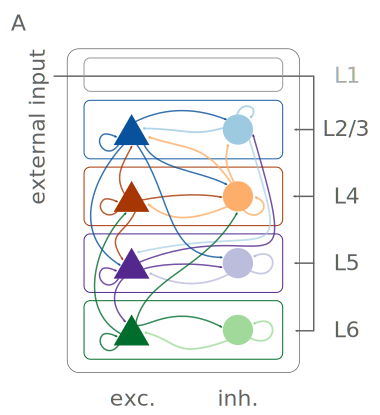
\includegraphics[width=\textwidth]{../figures/diagram_colored}
        \label{fig:diagram}
    \end{subfigure}
    \begin{subfigure}[b]{0.45\textwidth}
        \includegraphics[width=\textwidth]{\figdir population_size}
        \label{fig:population_size}
    \end{subfigure} ~
    \caption{
        Description of the network model. 
        (\textbf{A})~% 
        Diagram of the layered cortical network. 
        Layers 23, 4, 5, and 6 are composed of one excitatory
        (triangles) and one inhibitory population (circles) each.
        The connections are only shown for probabilities $>0.04$. 
        The external input is simulated by poissonian spike trains 
        and fed to all four layers containing populations. 
        Layer 1 does not contain neuron populations.
        (\textbf{B})
        Population sizes, total of 77169 neurons. The total number of inhibitory neurons is roughly
        $1 / 4$ of the number of excitatory neurons. 
    }
    \label{fig:model_description} 
\end{figure}
For each combination of pre- and postsynaptic population, pairs of neurons to be connected are drawn
randomly until a fixed number of synapses for each postsynaptic population is reached, 
allowing for multiple synapses and self-connections. 
Potjans and Diesmann's original model defines the connection probability $P_{\text{conn}, \,ab}$ 
of one neuron in the presynaptic population $a$ to form at least one connection with one neuron in 
the postsynaptic population $b$. For given population sizes $N_a$ and $N_b$, the number of 
synapses $C_{ab}$ is then calculated by
\begin{equation}
    C_{ab} = \frac{\ln \left( 1 - P_{\text{conn}, \,ab} \right)}{\ln \left( 1 - \frac{1}{N_a N_b} \right)} \, ,
    \label{eq:synapse_numbers}
\end{equation}
the inverse of the formula for connection probabilities of the original paper~\cite{potjans2014}.

The weight $w$ for each synapse is drawn from a normal distribution.
For excitatory presynaptic neurons, this mean value is set to $87,8$ pA (see below for 
a derivation). The mean for inhibitory ones is determined by multiplying 
with a factor $-g$, where the relative inhibitory synapse strength is set to 
$g = 4$. There is one important exception to this scheme:
The mean for the connection from L4e to L2/3e is increased by a factor of 
$j_{02} = 2$ (consult the corresponding paper~\cite{potjans2014} for details). 
The standard deviation is set to $10\%$ of the mean. 
The distributions from which weights are drawn are clipped, 
such that a neuron assigned to the excitatory 
population will not have associated outgoing synapses with $w < 0$ 
and vice versa for inhibitory ones. 
Delays are drawn from normal distributions as well, with a mean value 
of $1.5$ ms for excitatory presynaptic neurons and half this value for 
inhibitory ones. The relative standard deviation is set to $0.5$. The distributions
are again clipped such that $d \ge 0$

%\subsubsection{Neuron and synapse model}
The neurons are leaky integrate-and-fire neurons with a fixed voltage threshold. 
Below the threshold $\theta$, the dynamics of the membrane potential $V_i(t)$ 
for neuron $i$ are governed by the differential equation 
\begin{equation}
    \tau_\text{m} \,\frac{\text{d} V_i(t)}{\text{d} t} 
            = -(V_i(t) - E_\text{L}) + \frac{\tau_\text{m}}{C_\text{m}} I_i(t) \, .
    \label{eq:leaky_integrator}
\end{equation}
The membrane is specified by its resting potential $E_\text{L}$, 
its time constant $\tau_\text{m}$ and the capacitance $C_\text{m}$.
If, at time $t$, the threshold is reached, the neuron emits a spike and remains 
in a refractory period for a fixed time $\tau_\text{rp}$, with the membrane 
potential set to $V_\text{r}$ and discarding any input arriving. 
The total input to the neuron is represented by 
the current $I_i(t)$, which is a linear superposition of the individual 
postsynaptic currents (PSC) of the recurrent network.

The model implements  
postsynaptic current synapses with exponential shape, such that each 
spike arriving at one neuron leads to a current 
\begin{equation}
I_{\text{syn}}(t) = w \exp{\left(\frac{-t}{\tau_\text{syn}}\right)}	
    \label{eq:synaptic_current}
\end{equation}
where $w$ is the weight of the synapse in the model, given in pA
and $\tau_\text{syn}$ is the synapse time constant.
$w$ is identical to the amplitude of the PSC
at the time the spike arrives. 
Since measuring currents remains a difficult task for experimentalists, 
the model relays on measurements of the amplitude of the postsynaptic 
potential (PSP). In order to use the experimental observations%
\footnote{
Potential differences are much easier to access compared to incoming currents.
\emph{cite something?}
}, 
an approximative transformation is implemented 
by calculating the PSC induced if one spike with given PSP arrives at 
a neuron with membrane potential at rest. 
For $E_\text{L} = 0$, setting $I(t) = I_\text{syn}(t)$ in equation \eqref{eq:leaky_integrator}
yields:
\begin{equation}
    \dot{V}(t)
    = - \frac{1}{\tau_\text{m}} V(t) + \frac{w}{C_m} \exp{\left(-\frac{t}{\tau_\text{syn}}\right)} \,.
    \label{eq:psc_ode}
\end{equation}
This has the solution 
\begin{equation}
    V(t) =   
        - \frac{w \tau_\text{m} \tau_\text{syn}} {C_\text{m} \left(\tau_\text{m} - \tau_\text{syn}\right)}	
        \exp{\left( -\frac{t}{\tau_\text{syn}} \right)} 
        + C_1 \exp{\left(-\frac{t}{\tau_\text{m}} \right)}
    \label{eq:psc_ode_sol}
\end{equation}
with integration constant $C_1$.
With the boundary condition $V(t = 0) = 0$, this constant is set to
\begin{equation}
    C_1 = \frac{w \tau_\text{m} \tau_\text{syn}}{C_\text{m} \Delta\tau}	
    \label{eq:C_1}
\end{equation}
where $\Delta\tau := \tau_\text{m} - \tau_\text{syn}$ is introduced.
Thus
\begin{equation}
    V(t) = C_1 \left[\exp\left(-\frac{t}{\tau_\text{m}}\right) - \exp\left(-\frac{t}{\tau_\text{syn}}\right)\right]	\,.  
    \label{eq:V(t)}
\end{equation}
In order to get the PSP, we search for the maximum. Setting $\dot{V}(t) = 0$ 
yields
\begin{equation}
    t_\text{max} 
        = \ln{\!\left(\frac{\tau_\text{syn}}{\tau_\text{m}}\right)} 
            \left(\frac{1}{\tau_\text{m}} - \frac{1}{\tau_\text{syn}}\right)^{-1} \,.
    \label{eq:t_max}
\end{equation}
Inserting into equation \eqref{eq:V(t)} leads to 
\begin{equation}
    \text{PSP} := V(t_\text{max}) 
        = \frac{w \tau_\text{m} \tau_\text{syn}}{C_\text{m} \Delta\tau}	
            \left[ 
                \left( \frac{\tau_\text{syn}}{\tau_\text{m}} \right)^\frac{\tau_\text{syn}}{\Delta\tau} 
            - \left( \frac{\tau_\text{syn}}{\tau_\text{m}} \right)^\frac{\tau_\text{m}}{\Delta\tau} 
            \right] \,.
    \label{eq:PSP}
\end{equation}
For a given PSP, this equation is simply inverted in order to get the according 
weight $w$. In this model, the PSP for excitatory neurons is set to 0.15 mV, 
which yields a PSC of 87.8 pA. 
Finally, the 
input current of neuron $i$ can be described as the sum over currents induced by
arriving spike trains, 
\begin{equation}
    I_i(t) = \sum_j w_{ij} \sum_k \exp\left(\frac{t - t_j^k - d_{ij}}{\tau_\text{syn}}\right) \, ,
    \label{eq:input_current}
\end{equation}
where $t_j^k$ is the time the $k$-th spike by neuron $j$ was emitted and the 
delay between neuron $i$ and $j$ is set to $d_{ij}$. 

%\subsubsection{Model input, output and free parameters}
The model is solely driven by poissonian spike trains. Each neuron receives independent 
input at a rate specific to its population. This rate is determined by a global 
background rate of $8$ Hz multiplied by an external indegree $C_{a, \text{ext}}$ for
population $a$. This mimics a multiple number of synapses each transmitting the same input. 
At creation, the neurons are initialized by drawing their membrane potential from a normal
distribution with mean $-58$ mV and a standard deviation of $10$ mV. 
The activity of the network is measured in terms of spike trains (measuring the spike times 
of single neurons up to the maximal grid resolution $h$) and membrane potentials in mV. 
The results in this thesis are based on recording only a fraction of the neurons in the network, 
choosing the first $n_a$ neurons of each population $a$. Since no topology is applied, this is 
equal to choosing $n_a$ neurons to record from randomly. If not specified else, spikes are recorded 
from $1000$ neurons of each population, membrane potentials from $100$. The further analysis of the data 
is explained in following sections.
The large number of free parameters of the model and their chosen values are summarized in 
Table \ref{tab:network_params}. 
% Network parameters
\begin{table}[htpb]
    \centering
    \caption{
        Network parameters
        }
    \label{tab:network_params}
    \begin{tabular}{p{3.5cm}| *{8}{x{1.2cm}}}
        \rowcolor{TableColor}\multicolumn{9}{l}{Populations and input} \tn 
        Name $a$       
            & L2/3e & L2/3i & L4e & L4i & L5e & L5i & L6e & L6i  \tn \hline
        Population size, $N_a$   
            & 20683 & 5834 & 21915 & 5479 & 4850 & 1065 & 14395 & 2948 \tn
        Ext. inputs, $C_{a, \text{ext}}$ 
            & 1600 & 1500 & 2100 & 1900 & 2000 & 1900 & 2900 & 2100 \tn[0.1cm]
        Background rate     
        &&&& 8 Hz \tnn

        \rowcolor{TableColor}\multicolumn{9}{l}{Connection probabilities between pre- and postsynaptic populations} \tn
        \diagbox[width=3.9cm]{post~~~~}{pre~~~}&
              L2/3e & L2/3i & L4e & L4i & L5e & L5i & L6e & L6i  \tn \hline
        L2/3e
            & 0.101 & 0.169 & 0.044 & 0.082 & 0.032 & 0.000 & 0.008 & 0.000 \tn 
        L2/3i
            & 0.135 & 0.137 & 0.032 & 0.051 & 0.075 & 0.000 & 0.004 & 0.000 \tn 
        L4e
            & 0.008 & 0.006 & 0.050 & 0.135 & 0.007 & 0.000 & 0.045 & 0.000 \tn 
        L4i
            & 0.069 & 0.003 & 0.079 & 0.160 & 0.003 & 0.000 & 0.106 & 0.000 \tn 
        L5e
            & 0.100 & 0.062 & 0.051 & 0.006 & 0.083 & 0.373 & 0.020 & 0.000 \tn 
        L5i
            & 0.055 & 0.027 & 0.026 & 0.002 & 0.060 & 0.316 & 0.009 & 0.000 \tn 
        L6e
            & 0.016 & 0.007 & 0.021 & 0.017 & 0.057 & 0.020 & 0.040 & 0.225 \tn 
        L6i
            & 0.036 & 0.001 & 0.003 & 0.001 & 0.028 & 0.008 & 0.066 & 0.144 \tnn

        \rowcolor{TableColor}\multicolumn{9}{l}{Further connectivity} \tn
        $w \pm \delta w$    
            &  \multicolumn{3}{l}{$87.8 \pm 8.8 \,\text{pA}$}
            &  \multicolumn{5}{l}{Excitatory synaptic strengths} \tn
        $j_{02}$    
            &  \multicolumn{3}{l}{$2$}
            &  \multicolumn{5}{l}{Factor for connection L4e $\to$ L2/3e} \tn
        $g$    
            &  \multicolumn{3}{l}{$4$}
            &  \multicolumn{5}{l}{Relative inhibitory synapse strength} \tn
        $d_e \pm \delta d_e$    
            &  \multicolumn{3}{l}{$1.5 \pm 0.75 \,\text{ms}$}
            &  \multicolumn{5}{l}{Excitatory synaptic transmission delays} \tn
        $d_i \pm \delta d_i$    
            &  \multicolumn{3}{l}{$0.8 \pm 0.4 \,\text{ms}$}
            &  \multicolumn{5}{l}{Inhibitory synaptic transmission delays} \tnn

        \rowcolor{TableColor}\multicolumn{9}{l}{Neuron model} \tn
        $\tau_\text{m}$    
            &  \multicolumn{3}{l}{$10 \,\text{ms}$}
            &  \multicolumn{5}{l}{Membrane time constant} \tn
        $\tau_\text{ref}$    
            &  \multicolumn{3}{l}{$\hphantom{0}2 \,\text{ms}$}
            &  \multicolumn{5}{l}{Absolute refractory period} \tn
        $\tau_\text{syn}$    
        &  \multicolumn{3}{l}{$\hphantom{0}0.5 \,\text{ms}$}
            &  \multicolumn{5}{l}{Postsynaptic current time constant} \tn
        $C_\text{m}$    
            &  \multicolumn{3}{l}{$250 \,\text{pF}$}
            &  \multicolumn{5}{l}{Membrane capacity} \tn
        $E_\text{L}$    
            &  \multicolumn{3}{l}{$-65 \,\text{mV}$}
            &  \multicolumn{5}{l}{Leaky rest potential} \tn
        $V_\text{reset}$    
            &  \multicolumn{3}{l}{$-65 \,\text{mV}$}
            &  \multicolumn{5}{l}{Reset potential} \tn
        $\theta$    
            &  \multicolumn{3}{l}{$-50 \,\text{mV}$}
            &  \multicolumn{5}{l}{Fixed firing threshold} \tn
    \end{tabular}
\end{table}

%\subsubsection{Model validation}
In order to verify that the model behaves as assumed, a number of basic parameters 
is examined before stating more central results. As the implementation of the neuron model
is part of the NEST software and thus well established, the validation starts at the level 
of connections. Figure \ref{fig:syn_numbers} shows the number of synapses for each pair 
of pre- and postsynaptic population and 
the mean number of synapses each neuron receives from a specific population. The total number 
of synapses in the model is almost 0.3 billion synapses.  
\begin{figure}[htpb]
    \centering
    \includegraphics[width=0.8\linewidth]{\figdir syn_numbers}
    \caption{
        Connection between populations. (\textbf{A}) Visualization of 
        connection probability. (\textbf{B}) Calculated total synapse number between a pre- 
        and a postsynaptic population. These numbers are used for connecting the network, 
        using the connection rule "fixed\_total\_number". (\textbf{C}) Mean number of synapses
        a neuron in a specific postsynaptic population is receiving from all neurons of a 
        presynaptic population. These numbers are only applied when using the connection
        rule "fixed\_indegree" (for comparison between spiking network model and mean field theory).
    }
    \label{fig:syn_numbers}
\end{figure}
With the connection rule applied in the simulation ("fixed\_total\_number"~\cite{NEST}),
the number of synapses per postsynaptic neuron is expected to follow a binomial distribution:
for pre- and postsynaptic populations $a$ and $b$, respectively, 
each time a pair is drawn, one postsynaptic neuron is chosen with a probability 
$1 / N_b$, $N_b$ being the population size. This is repeated until $C_{ab}$ synapses are
created. 
Choosing this neuron exactly $k$ times and taking 
permutations into account then has the probability
\begin{equation}
    p_{\,\text{Binom}}\left(k; n=C_{ab}, p=\frac{1}{N_b}\right) = 
        {C_{ab}\choose{k}} 
        \left( \frac{1}{N_b} \right)^{k} 
        \left( 1 - \frac{1}{N_b} \right)^{C_{ab} - k} \,.
    \label{eq:binomial}
\end{equation}
Accordingly, the expected value of $k$ is $C_{ab} / N_b$. 
In Figure \ref{fig:syn_numbers_distribution}, the actual distribution of synapse numbers 
for the connection $L4e \to L4i$ is shown in a normalized histogram. 
The agreement between the numbers from the simulation and the theoretical expectation is quite
well. 
\begin{figure}[htpb]
    \centering
    \includegraphics[width=0.8\linewidth]{\figdir syn_numbers_distribution}
    \caption{
        Distribution of synapse numbers for the connection $L6e \to L6i$.
        The total number of synapses for this connection is $2888426$, 
        the mean number for each neuron in $L6i$ is $979$.
        The steps indicate the normalized histogram (bin width = 10) obtained 
        from a simulation, the dashed line is a binomial distribution, the 
        underlying distribution for the given connection rule. 
    }
    \label{fig:syn_numbers_distribution}
\end{figure}

To further validate the model on a basic level, a look at single neurons' membrane potentials 
is taken. Figure \ref{fig:single_membrane_potential} shows the membrane 
potentials of two neurons over the first 1.2 s of simulation and further 
the normalized histograms compared to the normalized histogram of a larger subset of the 
respective population. The neuron of the upper plots appertains to the population
$L6e$, the other one to population $L6i$. Potjans and Diesmann state that
these two populations have comparably low / high rates, the excitatory one firing at 
$\sim 1$ Hz, the inhibitory one at $\sim 7$ Hz~\cite{potjans2014}.
This is reflected in the average membrane potential which for the neuron of $L6e$
is much closer to the threshold $\theta = -50$ mV, whereas for the $L6i$ neuron, it is
closer to the resting potential $E_L = -65$ mV. Furthermore, it is observable, that a single 
neurons' membrane potential is not necessarily distributed as the population mean. 
This is due to the large variation in single neuron firing rates reported already in the 
original publication~\cite{potjans2014}. Observing the first 100 ms of the membrane potential 
indicates that the used initialization leads to a large hyperpolarization at least in these two 
sample neurons. Thus, for the further analysis, a transient period of 0.2 seconds is cut off the
data each time. 

\begin{figure}[htpb]
    \centering
    \includegraphics[width=0.8\linewidth]{\figdir single_membrane_potential}
    \caption{
        Membrane potentials of two exemplary neurons of the populations 
        $L6e$ (\textbf{A, C}) and $L6i$ (\textbf{B, D}). The data is taken from 
        a simulation of 1.2 s, recording the membrane potential every 1 ms. 
        In all four plots, the threshold $\theta = -50$ mV is indicated by a dashed line, 
        the resting potential $E_L = -65$ mV by a line of dashes and dots. 
        \quad (\textbf{A, B}) Membrane potential over the time of simulation. 
        The upper membrane potential reaches $\theta$ much more often than the lower one 
        (leading to a spike each time). The initial membrane potential 
        is drawn from a normal distribution.
        \quad (\textbf{C, D}) Normalized histograms of membrane potentials of the
        two neurons (thin steps) as well as the averaged ones for a subset of $100$ 
        neurons (thick steps). 
        Note that contributions due to neurons being in refractory 
        period after spiking are not removed, yielding peaks at $V_r = -65$ mV. 
    }
    \label{fig:single_membrane_potential}
\end{figure}



\subsection{Mean field model}
The derivation of a mean field theory goes along the 
lines of the work by Brunel~\cite{brunel2000}.
It starts of with a simplified model of 
$N$ leaky integrate-and-fire neurons. 
Each neuron receives input from the network by $C$ synapses, 
$C_E$ from excitatory and $C_I$ from inhibitory ones. 
Furthermore, each neurons receives $C_\text{ext} = C_E$ connections from 
external excitatory neurons.
The synapse numbers 
are determined by the relative size of the two populations through the factor
\begin{equation}
    \epsilon := \frac{C_E}{N_E} = \frac{C_I}{N_I} \,.
    \label{eq:epsilon}
\end{equation}
A central assumption is the sparsity of the network, expressed by $\epsilon \ll 1$.
Guided by anatomical estimates for the neocortex, the population sizes are set to
$N_e = 0.8N$ excitatory and $N_i = 0.2N$ inhibitory neurons. Taking the definition
\eqref{eq:epsilon}, this implies 
\begin{equation}
    C_I = \gamma C_E 	
 \label{eq:C_I}
\end{equation}
with $\gamma = 0.25$. The synaptic weights in this model are set to $J$ for 
excitatory presynaptic neurons and to $-g\, J$ for inhibitory ones, 
whereas the delays are fixed uniformly to $d$ for all synapses. 

At the heart of the mean field model
is the transition from the deterministic description of membrane potential 
dynamics to a probabilistic formulation. 
As in Potjans' model, the membrane potential follows
the differential equation \eqref{eq:leaky_integrator}. The input is simplified 
by implementing voltage based synapses which
yield an instantaneous and fixed change in membrane potential
for each spike arriving at the neuron instead of an exponential shaped PSC.
It can be described by a sum over Dirac delta-functions, 
\begin{equation}
    I_i(t) = \tau_\text{m} \sum_j J_{ij} \sum_k \delta(t - t_j^k - d_{ij}) \,.
    \label{eq:input_const_volt}
\end{equation}
The synaptic weights $J_{ij}$ in this case are equal to the PSP and given in mV.  
\emph{Multiple synapses between two neurons are excluded?!?}

A number of conditions are necessary in order to make the transition from 
this description to a probabilistic one:
\begin{itemize}
    \item The sparsity implies that 
        two neurons share only a small number of common input, such that pair correlations
        are negligible for $C / N \to 0$; 
    \item For the low single neuron firing rates $\nu$ compared to the 
        inverse membrane time constant $\tau_\text{a}$
        (e.~g. $\nu \sim10$ Hz and $1 / \tau_\text{m} \sim 1 / (20\,\text{ms}) = 50\, \text{Hz}$),
        a neuron receives a large number of small contributions per integration 
        time, each being very small compared to the threshold ($J \ll \theta$).
\end{itemize}
If these conditions are true, the input can be modeled as a time-varying average part
$\mu(t)$ plus a fluctuating gaussian part with amplitude $\sigma(t)\tau_\text{m}$:
\footnote{\emph{I have not yet understood the scaling by $\tau_m$...}}
\begin{equation}
    \frac{\tau_\text{m}}{C_\text{m}} \, I_i(t) =  \mu(t) + \sigma(t) \sqrt{\tau_\text{m}} \eta_i(t) \, .
    \label{eq:input_random}
\end{equation}
The random fluctuations are described by gaussian white noise $\eta_i(t)$ with 
$\langle  \eta_i(t)\rangle = 0$. The model explicitly excludes correlations, 
both in time and between different neurons, i.~e.
\begin{equation}
    \langle \eta_i(t) \: \eta_j(t') \rangle = \delta_{ij} \: \delta(t - t')	\, . 
    \label{eq:no_correlations}
\end{equation}
\emph{The latter assumptions has to be tested for the spiking model
that is to be described with this mean field approach.}

The fundamental parameter calculated by the mean field model is the single neuron
firing rate $\nu(t)$. In this basic model, it is assumed that any neuron of either 
of the two populations is firing with the same rate $\nu$ which is linked to the 
average input $\mu(t)$ by
\begin{equation}
    \begin{split}
        \mu(t)          &= \mu_l(t) + \mu_\text{ext} \\
        \text{with} \qquad \mu_l(t)        &= C_E \, J (1 - \gamma g) \nu(t - d) \tau_\text{m} \\
        \mu_\text{ext}  &= C_E J \nu_\text{ext} \tau_\text{m} \,.
        \label{eq:mu}
    \end{split}
\end{equation}
Similarly, for the amplitude of fluctuations $\sigma(t)$:
\begin{equation}
    \begin{split}
        \sigma^2(t)     &= {\sigma_l}^2(t) + {\sigma_\text{ext}}^2 \\
        \text{with} \qquad {\sigma_l}^2(t)       
                        &= C_E \, J^2 (1 + \gamma g^2) \nu(t - d) \tau_\text{m} \\
        {\sigma_\text{ext}}^2  &= C_E J^2 \nu_\text{ext} \tau_\text{m} \,.
        \label{eq:sigma}
    \end{split}
\end{equation}

Brunel then transforms equations \eqref{eq:input_random} and \eqref{eq:leaky_integrator}
into a Fokker-Planck equation describing the probability distribution of the membrane 
potential $P(V, t)$ in time: 
\begin{equation}
    \tau_\text{m} \, \frac{\partial P(V, t)}{\partial t} 
       \: = \: \frac{\sigma^2(t)}{2}  \: \frac{\partial^2 P(V, t)}{\partial V^2} 
         \: + \: \frac{\partial }{\partial V}  [(V- \mu(t)) P(V, t)] \, .
    \label{eq:fokker_planck}
\end{equation}
In the terminology of stochastic differential equations, the first term on the 
r.h.s. corresponds to a diffusion term originating in the fluctuations $\sigma$ 
of the input whereas the second part describes a drift due to the respective mean $\mu$ 
and the leaky quality of the neuron model. Introducing the probability current 
\begin{equation}
    S(V, t) 
    \: = \: - \frac{\sigma^2(t)}{2 \tau_\text{m}} \frac{\partial P(V, t)}{\partial V}  
        \: - \: \frac{V - \mu(t)}{\tau_\text{m}} P(V, t)
    \label{eq:prob_curr}
\end{equation}
through $V$ at time $t$ yields the continuity equation 
\begin{equation}
    \frac{\partial P(V, t)}{\partial t} \:=\: - \frac{\partial S(V, t)}{\partial V} \,.
    \label{eq:continuity}
\end{equation}

The probability distribution is subject to a number of 
constraints: Since the spiking resets neurons to $V_\text{rp} < \theta$, 
the membrane potential is always below this threshold:
$P(V, t) = 0$ for $V > \theta$. Infinite probability currents are excluded 
such that $P(V, t)$ must be continuous at any point. Specifically, 
this continuity forbids infinity spiking probabilities at the threshold $\theta$. 
The resulting constraint is 
\begin{equation}
    P(\theta, t) = 0 \,.
    \label{eq:continuity} 
\end{equation}
The probability current at the threshold is equal to the firing rate
$\nu(t)$. Inserting both $S(\theta, t) = \nu(t)$ and the above constraint into 
equation \eqref{eq:prob_curr} yields
\begin{equation}
    \frac{\partial P(\theta, t)}{\partial V}    
        = - \frac{2 \nu(t) \tau_\text{m}}{\sigma^2(t)}  \,.
\end{equation}
Neurons that fired at time $t$ come out of their refractory period at 
time $t + \tau_\text{rp}$ at the reset potential $V_\text{r}$. This leads to
a difference in probability current below and above $V_\text{r}$ proportional to 
the rate of neurons firing at $t - \tau_\text{rp}$ expressed by
\begin{equation}
    \frac{\partial P(V_r^+, t)}{\partial V} \: -  \: \frac{\partial P(V_r^-, t)}{\partial V} 
        = - \frac{2 \nu(t - \tau_\text{rp}) \tau_\text{m}}{\sigma^2(t)} \,.
\end{equation}
Finally, $P(V, t)$ is assumed to converge sufficiently quickly to zero:

\begin{equation}
\lim_{V \to -\infty} P(V, t) = 0 \, ;
    \quad 
    \lim_{V \to -\infty} V P(V, t) = 0 \,.
\end{equation}

A stationary solution $P(V, t) = P_0(V)$ with constant 
single neuron firing rate $\nu_0$ 
satisfying the above boundary conditions is then presented:
\begin{equation}
    P_0(V) = 2 \frac{\nu_0 \tau_\text{m}}{\sigma_0} 
        \exp{\left(- \frac{(V - \mu_0)^2}{{\sigma_0}^2} \right)}
        \int_{\frac{V - \mu_0}{\sigma_0}}^{\frac{\theta - \mu_0}{\sigma_0}} \! 
            \Theta \left(u - \frac{V_r - \mu_0}{\sigma_0} \right) e^{u^2} \, \text{d}u  \,. 
    \label{eq:P_V_0}
\end{equation}
Here, $\Theta(x)$ is the Heaviside step function, i.~e. 
\begin{equation}
    \Theta(x) = \begin{cases} 1 & \text{if } x \le 0 \\ 0 & \text{else } \end{cases}  \,.
    \label{eq:heaviside}
\end{equation}
The stationary mean input and fluctuation amplitudes are obtained by inserting 
$\nu_0$ into the equations \eqref{eq:mu} and \eqref{eq:sigma}, yielding 
\begin{align}
    \mu_0 	    &= C_E J \:\tau_\text{m} [\nu_\text{ext} + \nu_0(1 - g \gamma)]  \,, \\ 
    \sigma_0 	&= C_E J^{\,2} \,\tau_\text{m} [\nu_\text{ext} + \nu_0(1 + g^2 \gamma)] \,.
    \label{eq:mu_sigma_0}
\end{align}

In order to interpret $P(V, t)$ as a probability distribution, it is required to
satisfy the normalization condition
\begin{equation}
    \int_{-\infty}^{\theta} \! P(V, t) \, \text{d}V  + p_r(t) = 1 \, ,
    \label{eq:P_V_prob}
\end{equation}
where 
\begin{equation}
    p_r(t) := \int_{t - \tau_\text{rp}}^{t} \! \nu(u) \, \text{d}u 
    \label{eq:p_r}
\end{equation}
is the probability of neurons being the in refractory period.
In the constant case, this is simply 
\begin{equation}
    p_r(t) = p_{r, 0} = \nu_0 \tau_\text{rp}  \,.
    \label{eq:p_r_0}
\end{equation}

Inserting both $P_0(V)$ and $p_{r, 0}$ into the self-consistent condition \eqref{eq:P_V_prob}
then leads to an expression for $\nu_0$:
\begin{equation}
    \begin{split}
        \frac{1}{\nu_0} 	
            &= \tau_\text{rp} + \frac{1}{\nu_0} \int_{-\infty}^{\theta} \! P_0(V) \, \text{d}V  \\ 
            &= \tau_\text{rp} + \frac{2 \tau_\text{m}}{\sigma_0} 
                \int_{-\infty}^{\theta} \! \left[ 
                    \exp{\left(- \frac{(V - \mu_0)^2}{{\sigma_0}^2} \right)}
                    \int_{\frac{V - \mu_0}{\sigma_0}}^{\frac{\theta - \mu_0}{\sigma_0}} \! 
                        \Theta \left(u - \frac{V_r - \mu_0}{\sigma_0} \right) e^{u^2} \, \text{d}u 
                    \right] \, \text{d}V  \\ 
            &= \tau_\text{rp} + \frac{2 \tau_\text{m}}{\sigma_0} 
                \int_{\frac{V_r - \mu_0}{\sigma_0}}^{\frac{\theta - \mu_0}{\sigma_0}} \! 
                    \left[ 
                        e^{u^2}
                        \int_{-\infty}^{u \sigma_0 + \mu_0} \! 
                        \exp{\left(- \frac{(V - \mu_0)^2}{{\sigma_0}^2} \right)}
                        \, \text{d}V
                    \right] \, \text{d}u  \\ 
            &= \tau_\text{rp} + 2 \tau_\text{m}
                \int_{\frac{V_r - \mu_0}{\sigma_0}}^{\frac{\theta - \mu_0}{\sigma_0}} \! 
                    \left[ 
                        e^{u^2}
                        \int_{-\infty}^{u} \! e^{v^2} \, \text{d}v
                    \right] \, \text{d}u  \\ 
            &= \tau_\text{rp} + \tau_\text{m} \sqrt{\pi}
                \int_{\frac{V_r - \mu_0}{\sigma_0}}^{\frac{\theta - \mu_0}{\sigma_0}} \! 
                e^{u^2} \left(1 + \text{erf}(u)\right)
                \, \text{d}u  
        \label{eq:self_consistency}
    \end{split}
\end{equation}
This equation can be solved numerically for varying parameters as done by Brunel in order to 
characterize the different states the system can be found in. 

In order to transfer these results to the model of the neocortical microcircuit, 
the contributions to the input have to be adapted for each population. Instead of 
parametrized $\mu_0$ and $\sigma_0$ in terms of the variables $C_E$, $J$, $g$ and $\gamma$, 
a matrix notation as in equation \eqref{eq:synapse_numbers} is used: 
Synapse numbers and weights are defined as $C_{ab}$ and $J_{ab}$, respectively, 
where $a$ is the postsynaptic and $b$ the presynaptic population. 
Finally, the external input is written in a similar notation: 
An external excitatory population with single neuron firing rate $\nu_\text{ext}$ 
is connected to a neuron in population $a$ by 
$C_{a, \text{ext}}$ synapses of weight $J_{a, \text{ext}}$.
Including these definitions, the mean input and fluctuation amplitude can 
be written as 
\begin{align}
    \mu_a        &= 
        \tau_\text{m} \sum_{b \,\in \,\text{pop.}} C_{ab} \, J_{ab} \, \nu_b 
        + \tau_\text{m} C_{a, \text{ext}} \, J_{a, \text{ext}} \, \nu_\text{ext} \, ; \\
    {\sigma_a}^2 &= 
        \tau_\text{m} \sum_{b \,\in \,\text{pop.}} C_{ab} \, {J_{ab}}^2  \, \nu_b
        + \tau_\text{m} C_{a, \text{ext}} \,{J_{a, \text{ext}}}^2 \,\nu_\text{ext}\,,
\end{align}
where the sums go over all internal populations. In this specific case of eight 
populations one thus obtains eight equations for the 
firing rate $\nu_a$ of a single neuron in population~$a$, 
\begin{equation}
    \frac{1}{\nu_{a}} = \tau_{rp} 
        + \tau_\text{m} \sqrt{\pi}
            \int_{\frac{V_r - \mu_{a}}{\sigma_{a}}}^{\frac{\theta - \mu_{a}}{\sigma_{a}}} 
                e^{u^2} \left(1 + \text{erf}(u)\right) \,\text{d}u  \,.
    \label{eq:self_consistency_a}
\end{equation}
These equations are coupled by the boundaries of the integrals. Note that the index $0$ 
is omitted to facilitate readability, as the results are only concerned with stationary
solutions. After the rates $\nu_a$ are found, theses values can also be 
plugged into an equation for the distribution of membrane potentials. Extending the 
corresponding expression \eqref{eq:P_V_0} to more populations and again dropping the 
index $0$ yields
\begin{equation}
    P_a(V) = 2 \frac{\nu_a \tau_\text{m}}{\sigma_a} 
        \exp{\left(- \frac{(V - \mu_a)^2}{{\sigma_a}^2} \right)}
        \int_{\frac{V - \mu_a}{\sigma_a}}^{\frac{\theta - \mu_a}{\sigma_a}} \! 
            \Theta \left(u - \frac{V_r - \mu_a}{\sigma_a} \right) e^{u^2} \, \text{d}u  \,.
    \label{eq:P_V_a}
\end{equation}
In a reasonable regime, this function resembles a gaussian curve with discontinuity in the first 
derivative at $V_r$ (a visible "kink" or "step").
Ultimately, the model also makes a prediction about the regularity of single spike 
trains. For neurons firing irregularly, the interspike intervals
(ISI, i.~e. the difference in times between two successive spikes of one neuron) 
a distributed broadly. Hence, one parameter to measure irregularity is the coefficient 
of variation (CV) of ISI, defined as
\begin{equation}
    %c_{v, \text{ISI}} 
    \text{CV of ISI} = \frac{\sigma_\text{ISI}}{\mu_\text{ISI}} \,,
    \label{eq:cv_isi}
\end{equation}
where $\sigma_\text{ISI}$ and $\mu_\text{ISI}$ are the standard deviation and mean of 
the ISI. For the mean field theory introduced above, this quantity can be calculated
independently for each population. For the given parameters $\nu_a$, $\mu_a$ and 
$\sigma_a$ as in equation \eqref{eq:self_consistency_a}, the corresponding 
result~\cite{brunel2000} is
\begin{equation}
    (\text{CV of ISI})^2 
        = 2 \pi \left(\frac{\nu_a}{\tau_\text{m}}\right)^2
            \int_{\frac{V_r - \mu_{a}}{\sigma_{a}}}^{\frac{\theta - \mu_{a}}{\sigma_{a}}} 
            e^{x^2}  \,\text{d}x  \,
            \int_{-\infty}^{x} 
            e^{u^2} \left(1 + \text{erf}(u)\right)^2 \,\text{d}u  \,.
    \label{eq:CV_ISI_mf}
\end{equation}

\emph{What is irregular? Are there experimental estimates for CV of ISI?}



 
\subsection{Implementation, numerics and analysis}
\label{subsec:analysis}
The simulations are implemented with the NEST simulation tool using its python interface
pyNEST~\cite{NEST}. The differential equations of the network are solved with a computational 
step size of $h=0.1$, applying a numerical method known as "exact integration"~\cite{rotter1999exact}.
Numerical solving as well as the analysis of the data is done in using 
python~\cite{python} and heavily relies upon the numpy-scipy framework~\cite{scipy}. 
Plots are created using matplotlib~\cite{matplotlib}, 
colors are chosen based on ColorBrewer~\cite{brewercolor}.
The source code both for simulation and analysis can be reviewed at my
github server~\cite{ba_github} or more conveniently with the 
\textit{ipython notebook viewer}~\cite{notebook_viewer}.

The core part of the mean field theory constituted of the 
coupled integrals of equation \eqref{eq:self_consistency_a} relies on numerical
solving. The implementation of $\text{erf}(u)$ has a limited domain for the applied 
precision, such that for large values $u > 0$, the evaluation of 
$\text{erf}(\pm u)$ yields exactly $\pm 1.0$. For negative values, the integrand 
\begin{equation}
    f(u) = e^{u^2} \left(1 + \text{erf}(u)\right)
    \label{eq:integrand}
\end{equation}
thus becomes zero. In order to avoid this 
numerical error, the series expansion 
\begin{equation}
    f_\text{Laurent}(u) = 
        \frac{1}{\sqrt{\pi}} 
        \left( \frac{1}{u} - \frac{1}{2u^3} + \frac{3}{4u^5} - \frac{15}{8u^7} \right) +  
        \mathcal{O}\left( \frac{1}{u^9} \right) 
    \label{eq:expand_integrand}
\end{equation}
of $f(u)$ at $u = -\infty$ is applied whenever $u < -4$. 

A solution is not necessarily found for any initial guess. In order to achieve convergence, two possibilities 
can be applied: In the case of rates known from simulation, these serve as an initial guess. 
A test with simulated rates from 20 independent simulations for 20 seconds each lead to convergence%
\footnote{convergence is here defined by a maximum relative distance 
    $\|\boldsymbol\nu_{i + 1} - \boldsymbol\nu_i\| / \|\boldsymbol\nu_i\| \le 10^{-13}$ between two 
    successively computed vectors $\boldsymbol\nu_i$ with entries $\nu_{i, a}$~\cite{scipy}} % 
after a number of $42 \pm 12$ steps (mean and standard deviation). 
The second solution entirely independent of simulation data is solving the simplified model 
with only two populations corresponding to equation \eqref{eq:self_consistency} first.
Testing showed that convergence is found for a much broader range of initial guesses (data not shown).
The model can then be split 
into eight populations and all parameters can be iteratively transformed to the ones of the 
model in question. 

Most of the analysis does not require any specification at this point. 
However, the evaluation of membrane potentials of simulated neurons requires a specific treatment 
for neurons residing in refractory period at the $V_\text{r} = -65$ mV. 
Each neuron $i$ of population $a$ with firing rate $\nu_{a, i}$ measured over 
a recording time $T$ spends a time of \:$T \tau_\text{rp} \,\nu_{a, i}$\: in refractory 
period. If $T$ is divided into $n_T$ time bins, this corresponds to 
$n_T \, \tau_\text{rp} \,\nu_{a, i}$ time bins. The total number of entries 
corresponding to neurons in refractory period $n_{tot, \,\text{rp}, \,a}$ is then 
calculated by summing over all neurons, i.~e.
\begin{equation}
    n_{tot, \,\text{rp}, \,a}
        = n_T \, \tau_\text{rp} \,\sum_{i = 1}^{n_\text{rec}}\nu_{a, i} \, .
    \label{eq:n_tot_rp}
\end{equation}
This number is subtracted from the bin at $V_\text{m} = E_L$. Normalization is then
achieved by dividing each entry by the factor $n_T \, n_\text{rec} \, \Delta V_\text{m}$, 
with the bin widths $\Delta V_\text{m}$ of the voltage histogram.


\section{Results}
\label{sec:results}

\subsection{Spiking network model}
The simulation of the spiking network model will be analyzed in the following manner. 
At first, the results are directly compared to those obtained by the original 
model of Potjans and Diesmann. Both simulations are run for the same parameters, 
differences arise solely due to internal differences in assigning the random 
number generators. It is therefor not feasible to do a direct (spike per spike) 
comparison. Instead, a statistical description is chosen which furthermore sheds light
onto the differences between individual realizations with different seeds for the 
random number generators. Certain aspects such as
the distribution of single neuron firing rate within the population, 
the interspike interval distributions and the global population activity 
are then analyzed more thoroughly. Some of these  results are compared with 
theoretical approximations, namely the resulting distributions 
for Poisson processes.

A comparison between the pyNEST implementation and the original one written in SLI
is first supplied in form of raster plots (Figure~\ref{fig:raster_plot}), 
showing the activity of a subset of the neurons simulated for 400 ms 
after a transient period of 100 ms. The subset shown consists of the first 
$2.5 \%$ of the neurons created during the creation of the network. 
Both results have a very similar structure: Common features are the observable low 
rates of populations $L2/3e$ and $L6e$ as well some signs of synchrony within populations. 
Single neurons fire at a rate much lower than the activity of the 
entire population, as would be expected for networks in the AI regime \cite{brunel2000}. 
\begin{figure}[htpb]
    \centering
    \includegraphics[width=1.0\linewidth]{\figdir raster_plot}
    \caption{Raster plot showing spontaneous activity of network for 
        (A) the pyNEST implementation and (B) the SLI implementation.
        The simulation and network parameters for both simulations are 
        the same. 
        For each layer, the excitatory population is the upper one shown 
        (total of 1924 neurons) for $400$ ms (with a transient period of 100 ms). 
    }
    \label{fig:raster_plot}
\end{figure}

A more thorough comparison is done on the bases of three statistical quantities: 
Figure~\ref{fig:spontaneous_activity} shows the population means of single neurons firing rates, 
the coefficient of variation of interspike intervals (CV of ISI) as well as a measure for synchrony for both 
simulations. All parameters were calculated from $10$ repetitions of a simulation for 
$60.2$ s. Spikes were recorded from $1000$ neurons of each population, with recording 
starting after a transient period of $0.2$ s. 
For all three aspects, the agreement between the two implementations is very good 
and well within statistical fluctuations. 
The means are obtained by calculating the single neuron firing rates as 
the number of spikes measured over the time measured and then taking the mean over the entire population. 
\emph{ASSUMPTION: The box plot further shows that 
fluctuations relative to the mean are roughly equal for all populations, with outliers lying 
up to $\pm 10 \%$ above or below the median. Thus, the highest absolute fluctuations are observed 
for the layers $L5e, L5i$ and $L6i$.} 

The CV of ISI is calculated for each neuron that fired more than twice.
Although the results of both implementations agree, there is a disagreement with the results presented 
in the original paper, where a CV of ISI larger 0.8 for all populations is stated
under similar simulation conditions\cite{potjans2014}. 
This might be due to a difference in calculating the CV of ISI, for instance excluding neurons 
with particularly low firing rates. 
Especially 
for the populations with low rates ($L2/3e, L6e$), the finite simulation time leads to an estimation bias
of the CV of ISI as a significant ratio of the neurons in the population is either not included at all 
($n_i < 2$) or the part of the distribution covering higher CV of ISIs is not represented well~%
\cite{grun2010analysis}. 
\\\emph{IS THERE anything to be said about fluctuations?}

The synchrony measure explores the activity of each population as a whole. The respective population
activity is calculated by subdividing the time of measurement into equal bins (bin width = $3$ ms) 
and counting the number of spikes within each bin for each population. 
Dividing the variance by the squared mean yields the synchrony measure. 
A population firing totally asynchronously would yield a synchrony of zero as there would 
be no global oscillations i.~e. zero variance observed.
As with the CV of ISI, the results of both implementations agree, but do not reproduce the ones stated 
by Potjans and Diesmann \cite{potjans2014}. 
\\\emph{CAN THIS be traced back to the fact that they used 
only 5 s of simulation? -> methods: check synchrony for measurement time and bin width!}. 
\begin{figure}[htpb]
    \centering
    \includegraphics[width=1.0\linewidth]{\figdir spontaneous_activity}
    \caption{
        Derived statistical quantities for spontaneous activity of network for
        (\textbf{A - C}) the pyNEST implementation and (\textbf{D - E}) the SLI implementation, 
        using the same simulation and network parameters.
        Each implementation is run $20$ times independently, 
        measuring 1000 spike trains of each population in a simulation for 60 s 
        after a transient period of 0.2 s. 
        Statistical fluctuations 
        are indicated by the interquartile ranges (boxes extend to Q1 and Q3). 
        The median is indicated by a black line, the population mean by a star and 
        whiskers extend to 1.5 IQR (outliers indicated by crosses). 
        \quad (\textbf{A, D}) 
        \quad (\textbf{B, E}) Population mean of Coefficient of variation (CV) of interspike intervals (ISI) indicating 
        the irregularity of single neuron spiking. 
        \quad (\textbf{C, F}) Synchrony of the recorded subset of each population quantified by the 
        variance of the summed spike count histograms (bin width 3 ms) divided by
        its mean. 
    }
    \label{fig:spontaneous_activity}
\end{figure}

In order to get a deeper insight into the dynamics of the simulated network, the single neuron firing 
rates and the CV of ISI of single neurons are examined in Figure \ref{fig:single_neuron_activity}.
The observed fluctuations around the population mean are remarkably large especially when compared 
to the fluctuations of the population mean for different realizations. This can be interpreted as 
an indication that the population rates depend strongly on averaged input and connection numbers
and less on the actual wiring, i.~e. that a mean field approach would be able to capture the main features 
of first order quantities. 
\begin{figure}[htpb]
    \centering
    \includegraphics[width=1.0\linewidth]{\figdir single_neuron_activity}
    \caption{
        Firing rates (\textbf{A}) and CV of ISI (\textbf{B}) for single neurons. 
        The data is take from one simulation of the pyNEST implementation 
        simulating $60$ s after a transient period of 0.2 s and measuring 
        $1000$ neurons of each population. The symbols of the box plot 
        are similar to the ones of Figure \ref{fig:spontaneous_activity} 
        (boxes: Q1-Q3, median:black line, mean: star, 
        whiskers to 1.5 of IQR, outliers: crosses). 
        \\\emph{DISCUSSION?
        Both quantities show very large fluctuations. One of the suspected
        causes is the connection rule applied, yielding a binomial distribution 
        of synapse numbers within one population
        such that differences in input between single neurons can be 
    considerably large.}
    }
    \label{fig:single_neuron_activity}
\end{figure}

\emph{MORE DETAILED view on results:
Synchrony of populations in terms of population activity, 
see Appendix, Figure \ref{fig:population_activity}. 
The observed global oscillation indicates non-negligible correlations
and thus contradicts the assumption of uncorrelated gaussian white noise 
(in the mean field model).}

\subsection{Mean field theory}
The primary results of the mean field theory cut down to the prediction of 
population mean of single neuron firing rates and then using these rates 
in order to predict the CV of ISI and the distribution of membrane potentials. 
These results are directly compared to 
the corresponding quantities recorded from the spiking network 
model simulation analyzed in the previous sections. 

The predicted firing rates obtained by solving equation 
\eqref{eq:self_consistency_a} are displayed in a bar plot in Figure 
\ref{fig:compare_sim_mf_fixed_total_number}. Rates measured in 
simulation and previously stated in Figure \ref{fig:spontaneous_activity}
are shown for comparison. As visible, the results of the mean field model 
match those of the simulation qualitatively: The sequence of populations 
ordered by increasing firing rates is reproduced with the exception of
the two highest rates, i.~e. the two populations of layer $5$. 
The most apparent difference is the seen for the populations firing at the lowest 
rates, $L2/3e$  and $L6e$. The measured rates are almost equal while the 
predicted rates are very different, $r_{L6e} = 1.6$ Hz is almost three times 
as large as $r_{L2/3e}$. Another observable feature is that the predicted rates
for six of the eight populations are smaller than the measured ones. 
The comparison can further be quantified: The difference 
$    \Delta r_a := r_{\text{mf}, a} - r_{\text{sim}, a} $
between the mean of simulated rates $r_{\text{sim}, a}$ and predicted rates 
$r_{\text{mf}, a}$ for each population $a$ is shown in table \ref{tab:diff_fixed_total_number}. 
For the absolute values of all populations, mean and standard 
deviation are $(0.46 \pm  0.13)$ Hz. The relative differences 
are much larger for populations firing at low rate.  
The CV of ISI for each population is the result of plugging in the predicted rates 
into equation \eqref{eq:CV_ISI_mf}. A comparison with simulation data is shown
in Figure \ref{fig:compare_sim_mf_fixed_total_number}. Here the result turns out 
to be quite close to the measured one. In all cases, the mean field theory predicts 
a slightly higher variability. The larges deviation is again seen in the populations 
$L2/3e$ and $L6e$, those firing at the lowest rates. Ignoring these two populations, 
the theory further predicts the order of variability among the populations, although
the differences are small. As for the rates, numerical results are subsumed in 
Table \ref{tab:diff_fixed_total_number}, using analogous definitions. 
Averaged over all populations, the deviation between mean field theory and simulation
is $(0.06 \pm 0.04)$ corresponding to about $(6 \pm 5) \%$. 
\emph{
    Discuss these results in Discussion: origin of discrepancies:
    bad agreement for j02 = 2; larger rates: origin?
    CV of ISI: reason for deviation at low rates: bias in measurement / correlation?
}

% Table of results of comparison
\begin{table}[htpb]
    \centering
    \caption{Difference between predicted and simulated population means for single 
    neuron firing rates; absolute and relative to simulated rates.}
    \label{tab:diff_fixed_total_number}
    \begin{tabular}{p{2.4cm}| *{8}{x{1.12cm}}}
        \rowcolor{TableColor}
        Population $a$       
        & L2/3e & L2/3i & L4e & L4i & L5e & L5i & L6e & L6i  \tn[0.2cm]
        $\Delta r_a$ / Hz
            & -0.41 & -0.61 & -0.38 & -0.36 &  0.37 & -0.70 &  0.54 & -0.32 \tn[0.2cm]
        $\Delta r_a \:/\: r_{\text{sim}, a}$
            & -0.42 & -0.20 & -0.09 & -0.06 &  0.05 & -0.08 &  0.49 & -0.04 \tn[0.2cm]
        $\Delta \text{CV}_a$
            &  0.14 &  0.05 &  0.04 &  0.03 &  0.02 &  0.03 &  0.13 &  0.03 \tn[0.2cm]
        $\Delta \text{CV}_a / \text{CV}_{\text{sim}, a}$
            &  0.16 &  0.06 &  0.05 &  0.03 &  0.02 &  0.04 &  0.15 &  0.04 \tn[0.2cm]
    \end{tabular}
\end{table}

% Comparison mean field / simulation
\begin{figure}[htpb]
    \centering
    \includegraphics[width=0.8\linewidth]{\figdir compare_sim_mf_fixed_total_number}
    \caption{
        Comparison between mean field theory and spiking network model. 
        Bars indicate the single neuron firing rates predicted by the mean field 
        theory, crosses the calculated ones of 20 simulation (as previously shown in
        Figure \ref{fig:simulation_activity}). The connection
        rule was set to "fixed\_total\_number".
        Comparison between mean field theory and spiking network model.
    }
    \label{fig:compare_sim_mf_fixed_total_number}
\end{figure}

Applying equation \eqref{eq:P_V_a} on the predicted rates yields the 
membrane potential distributions shown in 
Figure \ref{fig:membrane_potential}. 
The obtained distributions  are confronted with the normalized histograms of recorded 
membrane potentials of a subpopulation of $n_\text{rec} = 100$ neurons for 
each population. The contribution due to neurons in refractory period is removed
(see Analysis in Methods, \ref{subsec:analysis} for details). 
Similar to the firing rates, 
the agreement is quite good and the largest deviations are observable for  
the populations $L2/3e$ and $L6e$, corresponding to the lowest firing rates and
largest relative differences as calculated before. A common feature found for all
populations is that the predicted distributions are narrower than the recorded ones.
Furthermore, the predicted maximum is shifted towards the threshold. The effect
of neurons coming out of refractory period is underestimated in some cases, 
visible for example in populations $L2/3i$ and $L4i$ where the mean distributions 
show a step while the kink in the theoretical curves is hardly detectable. 
In the case of population $L5i$ and $L6i$, however, this behavior is captured well. 

% Membrane potentials
\begin{figure}[htpb]
    \centering
    \includegraphics[width=0.8\linewidth]{\figdir membrane_potential}
    \caption{
        Distribution of membrane potentials for each population. 
        Shown are both the results of simulation (histogram) and 
        the predictions of the mean field theory (continuous line). 
        The simulation results are histograms (bins width $\Delta V_\text{m} = 0.25$ mV) 
        of membrane potential recordings 
        of 100 neurons, recorded every 1.0 ms for a simulation time of 1.0 s 
        (after a transitional period of 0.2 s), 
        adjusted for neurons in refractory period (see text). 
        The binning in voltage is the same as applied in Figure 
        \ref{fig:single_membrane_potential}. 
        The voltage for neurons in refractory period $V_\text{r} = -65$ mV 
        is indicated by the dashed and dotted line. The threshold is at 
        $\theta = -50$ mV. 
    }
    \label{fig:membrane_potential}
\end{figure}

\subsection{Simulation closer to mean field theory }
In order to assess some of the discrepancies between the predictions of the mean field 
model and data from simulation, a number of parameters in the simulation are adjusted 
such that they resemble the ones chosen in the mean field theory more closely. 
Differentiating parameters in the previous comparison are listed in the 
Table~\ref{tab:diff_params}.
\begin{table}[htpb]
    \centering
    \caption{Parameters chosen differently between simulation and mean field model previously.}
    \label{tab:diff_params}
    \begin{tabular}{p{3.0cm} *{2}{|p{5.3cm}}}
        \rowcolor{TableColor}
        Parameter & Simulation & Mean field theory   \tn[0.2cm] 
        Network size &
            finite; $N_a$ & 
            none (neglecting finite size effects)
            \tn[0.1cm] %\hline
        Connection rule & 
        "fixed\_total\_number"; binomial distribution of synapse numbers & 
            "fixed\_indegree"; same synapse number per neuron 
            \tn[0.1cm] %\hline
        Synapse type & 
            current based &
            voltage based
            \tn[0.1cm] %\hline
        Synaptic weights & 
            clipped normal distribution & 
            Dirac delta distribution 
            \tn[0.1cm]
    \end{tabular}
\end{table}

\emph{Simulation with parameters adapted are on their way...}


\chapter{Discussion}
\label{sec:discussion}

% Spiking network
The reimplementation of Potjans and Diesmann's spiking network simulation  
confirmed the expectation: The original model's results were reproduced 
well within the statistical fluctuations. The fluctuations of the calculated population 
means between different instantiations of the model are 
relatively small, a characteristic that can be interpreted as an indication that a mean 
field approach is suited well for describing the corresponding network:
The parameters describing the main features of the network activity
depend strongly on average input and connection numbers,
and much less on the actual wiring.
However, this assertion has to be restricted to 
random networks, as more detailed structure, for example induce by learning, 
can lead to stronger effects of correlation (see for example \citeb{staude2010higher}).
For a single simulation, the fluctuations along neurons within one population
were shown to be large both for the firing rate and the 
CV of ISI. This can be tracked back to the large deviations of input between 
different neurons: Due to randomly choosing the synapses and adding further 
variability by distributing the synapse number (as shown for model validation, 
see Methods, \autoref{subsec:methods_simulation}), 
some neurons will receive more excitatory or inhibitory input than others 
and fire accordingly. 
Since the results reproduce those of the original study, the according characterization 
of the network holds as well: The network activity is labeled as asynchronous irregular, 
with a mean CV of ISI above 0.8 and the applied synchrony measure ranging from 
values below $2$ (populations L5i, L6e and L6i), up to $\sim 8$ for L5e.
Still, the larger values of synchrony indicate that the amount of correlation
might not be negligible for the spike rate. This has to be taken 
into account when interpreting the results of the mean field model. 

% Mean field theory
Introducing the mean field theory for the simulated spiking network 
turned out to be remarkably successful. 
The formal extension 
from the original model of two populations has been a rather small step, 
while the incorporation of further details as well as the numerical implementation 
revealed a number of obstacles. The resulting
algorithm, nonetheless, is a convenient and computationally inexpensive tool for 
predictions. It has been shown to predict central quantities 
of the network activity to a high degree of accuracy.  

% MF: Rates
The predicted single neuron firing rates differ by less than
$0.3$\,Hz for all populations but L5e ($0.6$\,Hz lower than measured). 
Except for the latter and L2/3e, the relative error is below $7\,\%$.
In most cases, the rates are slightly lower than the measured ones..
One reason for this underestimation could be the negligence of correlation: 
Larger correlations among excitatory input can lead to higher fluctuations 
and thus higher spiking rates~\cite{staude2010higher}. This 
assertion has to be taken with care, though, as correlation in inhibitory 
populations can cancel the effect \marginpar{(citation!! Sadra emphasized that)}. 

% MF: CV of ISI
The prognosis for the irregularity of spike trains, measured by the coefficient of
variation of interspike intervals (CV of ISI) turns out to be evenly accurate:
For all populations, the deviation between theory and simulation is of the order 
of $0.05$, the largest being observed for the populations L2/3e and L6e with $0.07$ 
and $0.08$. The latter ones are the populations firing at the lowest rate. 
The general overestimation of irregularity can be interpreted in two ways. 
One explanation for the remaining differences can be an estimation bias of the CV of ISI 
using spike trains of finite lengths arising as a significant ratio of the neurons in the 
population is either not included at all (if the number of spikes is $ < 2$) or the part of the 
distribution covering higher CV of ISI is not represented well (see \citeb{nawrot2010analysis} for 
details). This is especially critical for the populations with low rates (L2/3e, L6e), 
which indeed do show the largest deviations.
What cannot be accounted for by this bias would indicate a lower irregularity than that 
of the respective stationary Gaussian process, pointing towards temporal correlations
introduced for example by the synapse model beyond the effects accounted for
(see e.\,g. \citeb{brunel1999fast} for the case of $\alpha$ synapses in a simpler context). 

% MF: Membrane potentials
The third and last measure predicted by the mean field model, the distribution of 
membrane potentials, agrees well with the obtained simulation data, too. 
Both the shape and position of the distribution are reproduced.
The kink at the resting potential $V_\text{r}$ due to neurons exiting the 
refractory period is reproduced but less pronounced than the measured one, indicating that the diffusion
away from this point is slower than assumed. 
The maxima of the predicted distributions are slightly 
shifted towards the resting potential. 
Again, the interpretation of the distribution has to be done with care:
A lower maximum does not correspond to lower firing rates. 
The populations of layer 5 illustrate this: While for both, the shift in membrane 
potential is about equal, the excitatory firing rate is underestimated whereas the 
inhibitory one is overestimated. 
In the mean field model, this is reflected by relating the firing rate 
only to the probability current at the threshold $\theta$, not to the 
shape of the curve at other points (cf. \autoref{eq:prob_curr} and following).
Further, higher firing rates due to correlations are not detectable in the 
membrane potential distribution: 
Even if the membrane potential spends most time close to the resting potential, 
a large number of excitatory spikes arriving in a short time would lead to a quick rise and
firing without affecting the distribution significantly.  


% Summary of results, explanations and shortcomings
In summary, the hypothesis for the analytical ansatz is confirmed: 
The considered activity measures of the simulated spiking network model of the neocortex 
can be predicted by a mean field theory assuming uncorrelated Gaussian input.
Possible explanations for the remaining deviations are (i) correlations between neurons, 
yielding an input to single neurons different from the assumed white Gaussian noise;
(ii) temporal correlations induced by the synapse type different from the 
delta synapses of the mean field model; and finally (iii) fluctuations in the 
input of single neurons. 
%\emph{Comparison with simulations where the according parameters are adapted 
    %have show the individual effects}.

% Use of the theory, limits
The value of the analytical framework developed is twofold: On the one hand, 
it provides a useful tool for predicting the activity of a spiking network model
over a large range of parameters 
%\emph{as observed for external frequency $\nu_{ext}$ 
%and relative inhibitory synapse strength $g$}. 
On the other hand, it represents an
essential means for identifying relevant measures and understanding the emergent 
dynamics of the complex systems under consideration. This is a hard and one of the 
most important tasks in this field. 
The long lasting
debate over whether neural coding is rate based or exploits precise timing and correlations
may at some point be solved by
excluding one or the other option using a sensible framework
of biological data, spiking network simulation and analytical arguments. 
On a less ambitious scale, the presented models can at least indicate by how much 
correlations effect the observed rates. 

% Outlook
The presented combination of the spiking network model and the mean field approach
could serve as a framework to tackle further questions. 
The implementation in PyNEST could work as a convenient basis for extensions 
such as the inclusion of newly available experimental data.
Furthermore, different neuron populations, 
especially concerning different interneuron classes, may be included, 
making the simulation a viable means for testing hypothesis about their 
role. 
Another possible extension already introduced in the 
original model \cite{potjans2014} is unspecific input from a thalamic population. 
When applying this input for short bursts (e.\,g. 10 ms), 
this can by used in order to examine the way
increased spike rates are propagated 
along the different layers in time and thus assessing the 
path of information processing within the neocortex.
The mean field approach, however, would have to be extended to a non-equilibrium 
regime since it lacks temporal resolution at the present state. 
Finally, when focusing on neural computation, one might also include specific input.
An interesting context is orientation selectivity, using 
oriented input resulting in neuronal tuning curves.
To this end, the mean field approach can be extended to single neurons 
as implemented for example by ~\citeb{sadeh2015orientation} 
for the case of one excitatory and one inhibitory population.





\section{Endnotes}
\label{sec:endnotes}
I am indebted to Stefan Rotter and Benjamin Merkt for introducing 
me into the fascinating field of computational neuroscience, always
being open for questions and guiding when possible. 



\section{Bibliography}
\printbibliography[heading=subbibintoc]
\clearpage

\clearpage 
%\section{Appendix A: Source code}
We excluded the source code of the figures here in order to focus on the relevant algorithms; 
The figures used in the report are merely a visualization of the calculations. The full programs can
be reviewed at our github server~\cite{ba_github} or more conveniently with the \textit{ipython notebook viewer} 
\cite{notebook_viewer}.




\end{document}

